
\section{Part 3: Forward vs. Backward }
\label{sec: Part 2}

Previously, we examined how tie breaking for the same $f(n)$ value with the $g(n)$ value can lead to drastic differences in run times for \emph{Repeated Forward $A^*$ search}. In this section we will examine another variation in the \emph{$A^*$ search} algorithm.


Up to now, we have been examining \emph{Repeated Forward $A^*$ search}, where the path is planned starting from the agent to the goal. However, a variation, called \emph{Repeated Backward $A^*$ search} exists, which means that the path is planned from the goal to the agent, and then executed by the agent. Every time a new obstacle is in the path, the algorithm computes a new path from the goal to the agent. Below are the run times of comparing the two methods. In our tests, we consider a larger $g(n)$ value as the tie breaker, and after that, which ever node was placed first in the priority queue.

\begin{figure}[H]
  \centering
  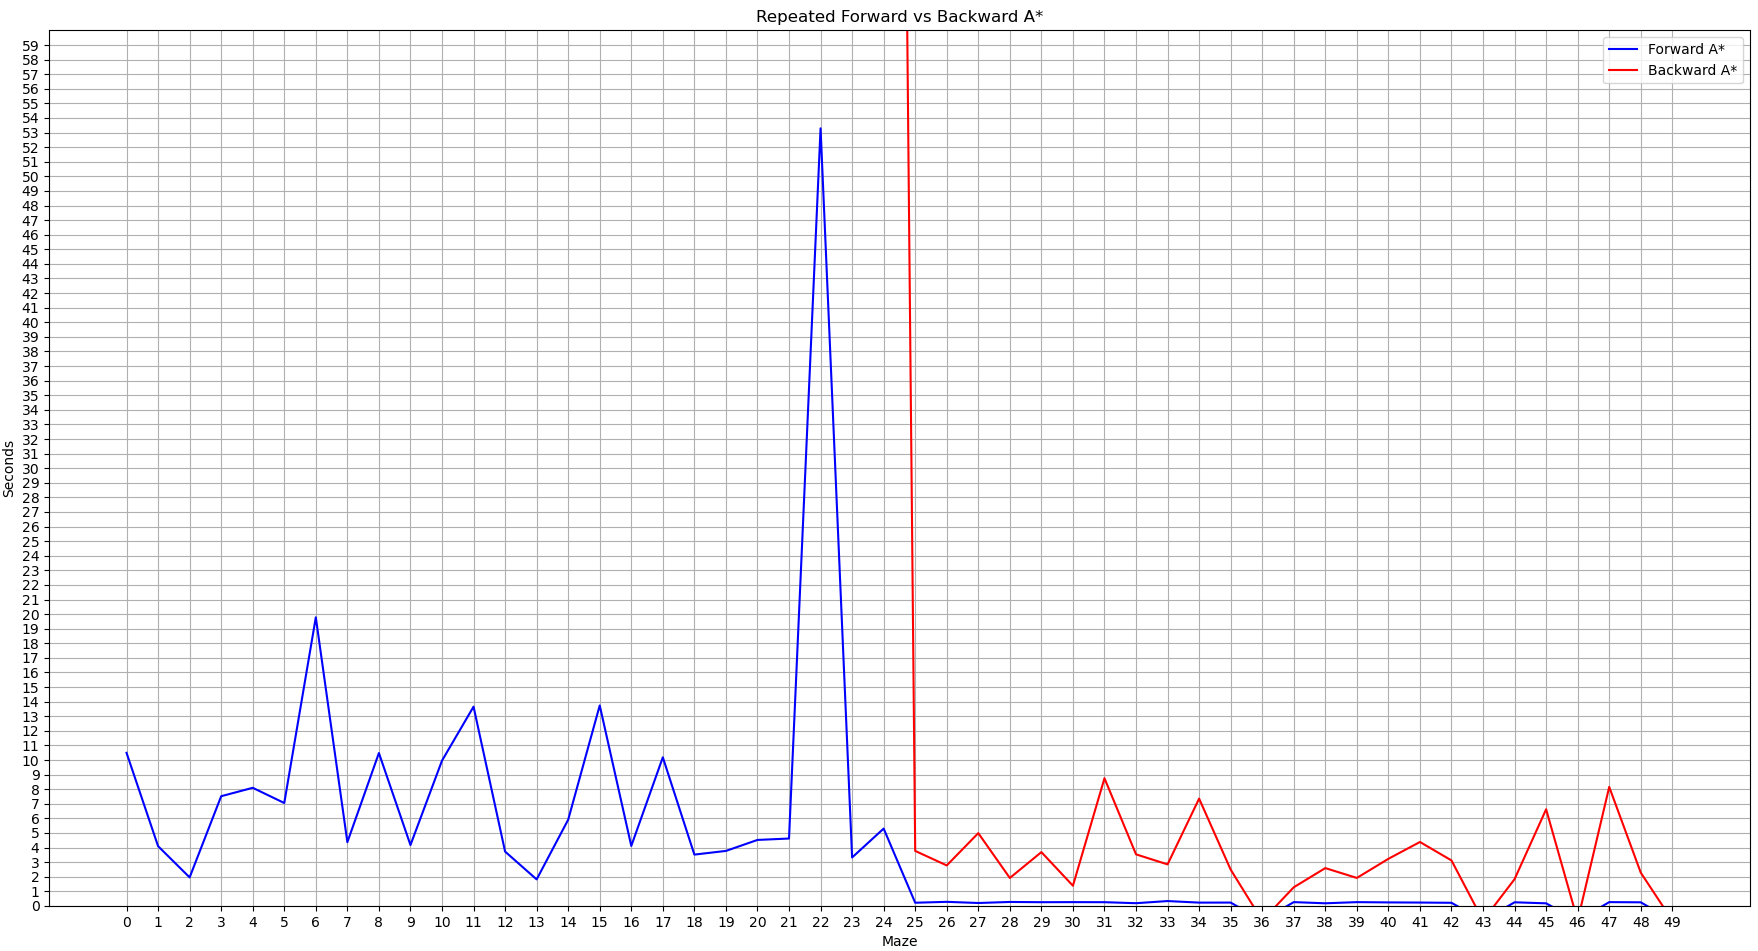
\includegraphics[width=1\linewidth]{Report/Part3/Figure_2.png}  
\caption{Repeated Forward vs Backward $A^*$ Comparison}
\end{figure}

Our results show that \emph{Repeated Backward $A^*$} performed significantly worst than \emph{Repeated Forward $A^*$}. For our backtracked mazes, the run times of \emph{Repeated Forward $A^*$} even surpassed 60 seconds, often over 200 seconds.


The reason for the long run times of \emph{Repeated Backward $A^*$} has to do with an observation we previously made. We saw in \emph{Figure 6} that as long as we have an open map and our start and goal are placed in a certain way (the same start and goal is chosen for all our tests), \emph{$A^*$ search} will act as a \emph{Depth First Search}. This was because all cells would have the same $f(n)$ value. However, in our mazes this is not the case. We have many walls, and therefore, $f(n)$ will alter for paths to many cells. 


Now how does this relate to the run times of Forward and Backward \emph{$A^*$ search}? In \emph{Repeated Forward $A^*$}, we perform a \emph{Depth First Search} from the start to the goal. As we move along and encounter walls, we recompute the path, and we will hit the wall very early in our search. This means all cells visited after passing the wall will all have the same $f(n)$ value and the rest of the algorithm will follow \emph{Figure 6}.


On the other hand, with \emph{Repeated Backward $A^*$} we will be computing a path from the goal to the start. This means after our first iteration, we will move until we meet a wall. Then, in our new computation of the path, our algorithm will compute a \emph{Depth First Search} until it meets the wall. Now here lies the problem. Since our \emph{Depth First Search} is from the goal to the start, and the wall is near our start, there are many nodes in our priority queue with smaller $f(n)$ values than the node that goes around the wall. So now, we must expand all of those nodes first, and then continue with the final path. 


\begin{figure}[H]
\begin{subfigure}{.5\textwidth}
  \centering
  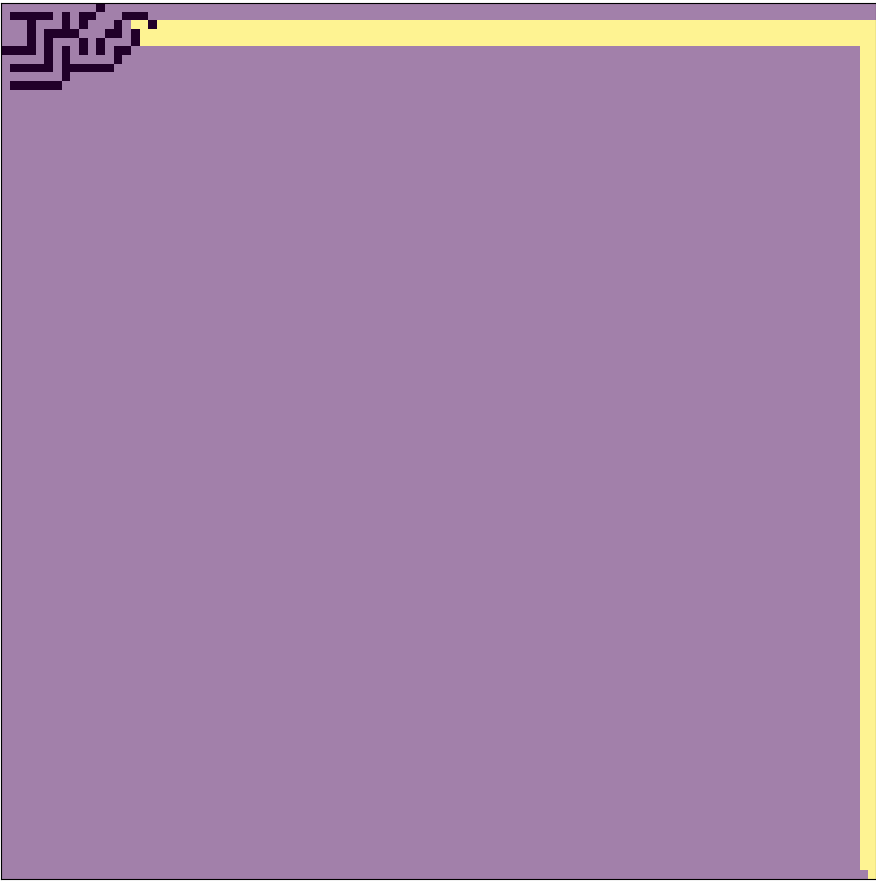
\includegraphics[width=0.8\linewidth]{Report/Part3/Forward_Astar_iter21.png}  
  \caption{Forward \emph{$A^*$ search}}
\end{subfigure}
\begin{subfigure}{.5\textwidth}
  \centering
  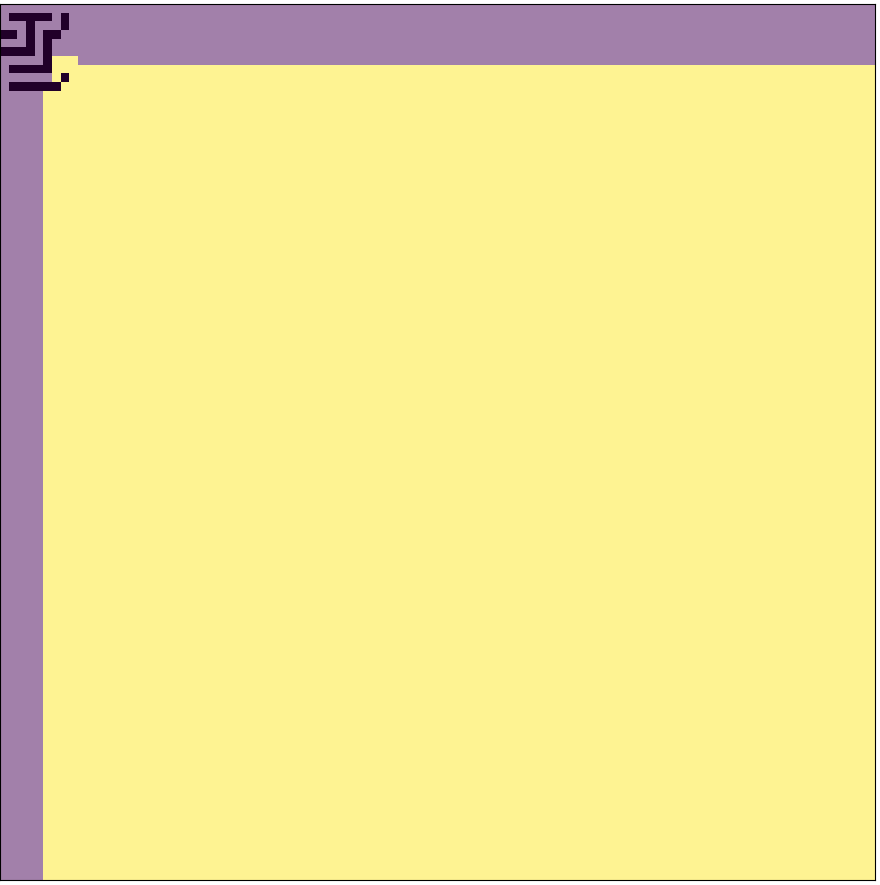
\includegraphics[width=0.8\linewidth]{Report/Part3/Backward_Astar_iter21.png}  
  \caption{Backward \emph{$A^*$ search}}
\end{subfigure}
\caption{The visited nodes of an iteration of $A^* search$}
\end{figure}


In essence, both variants of \emph{$A^*$ search} are actually the same. The only difference is where in our first \emph{Depth First Search} path the wall is located. The further the wall is located down the initial \emph{Depth First Search} path, will mean our search will take much longer then if we had reversed order. In general, you could think of it as the midpoint of the initial expanded path. If the obstacle is past one side of the path, \emph{Repeated Backward $A^*$} is better. And if the obstacle is on the other side of the midpoint, \emph{Repeated Forward $A^*$} will perform better.

\begin{figure}[H]
\begin{subfigure}{.5\textwidth}
  \centering
  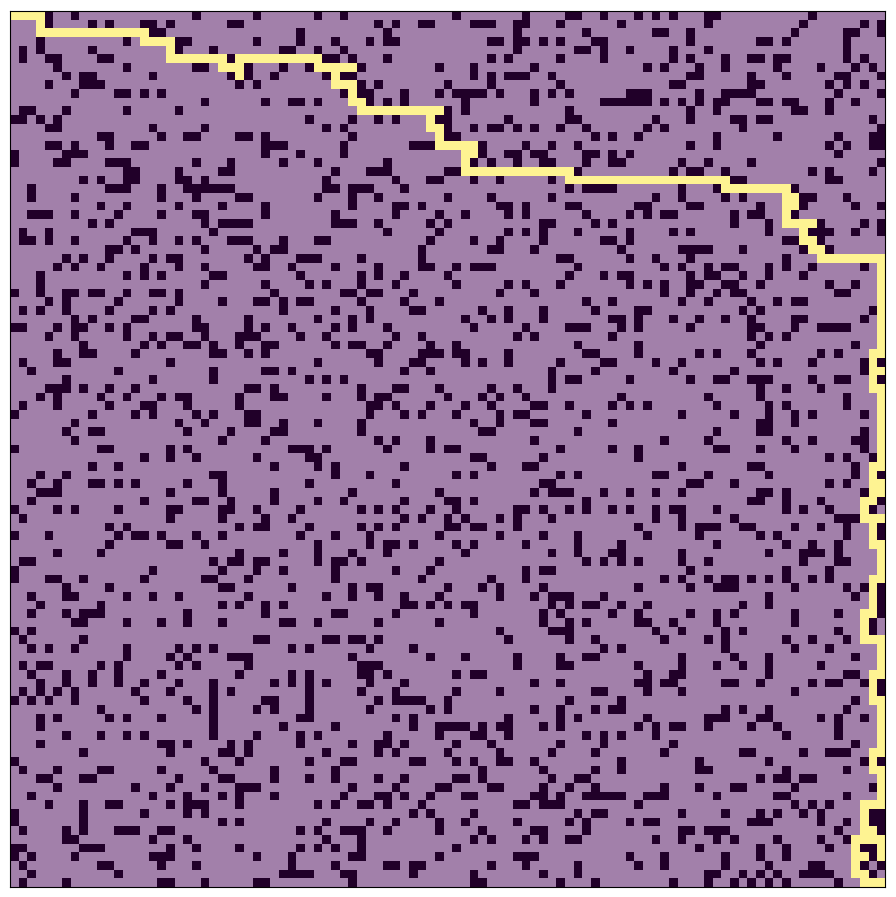
\includegraphics[width=0.8\linewidth]{Report/Part3/larger_g_forward_302.png}  
  \caption{Forward $A^*$, 302 nodes path length}
\end{subfigure}
\begin{subfigure}{.5\textwidth}
  \centering
  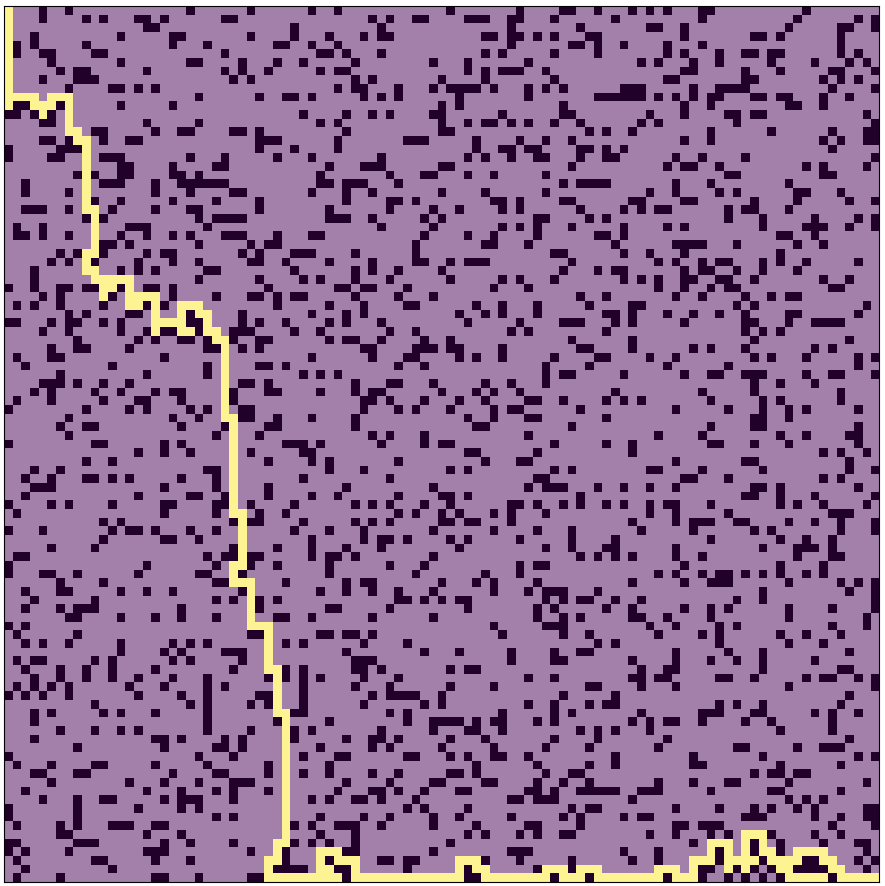
\includegraphics[width=0.8\linewidth]{Report/Part3/larger_g_backward_339.png}  
  \caption{Backward $A^*$, 339 nodes path length}
\end{subfigure}
\newline
\linebreak
\linebreak
\begin{subfigure}{.5\textwidth}
  \centering
  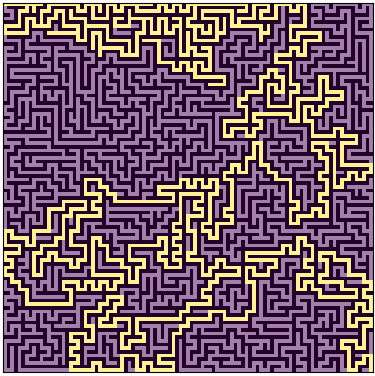
\includegraphics[width=0.8\linewidth]{Report/Part3/larger_g_forward_3178.png}  
  \caption{Forward $A^*$, 3178 nodes path length}
\end{subfigure}
\begin{subfigure}{.5\textwidth}
  \centering
  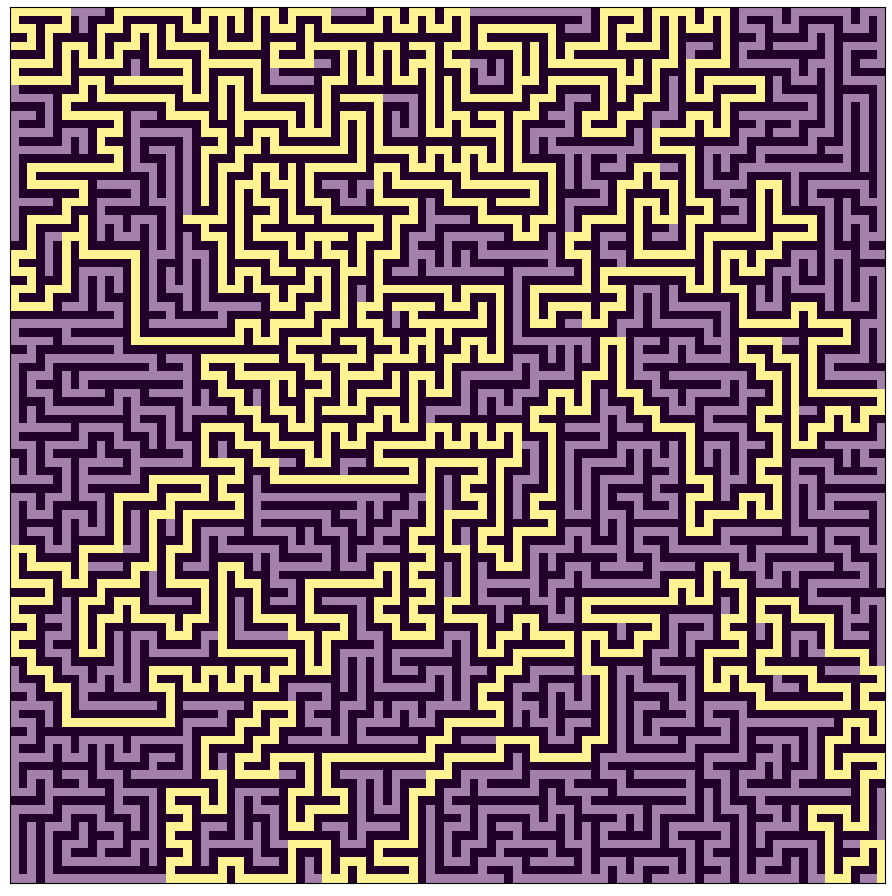
\includegraphics[width=0.8\linewidth]{Report/Part3/larger_g_backward_4861.png}  
  \caption{Backward $A^*$, 4861 nodes path length}
\end{subfigure}
\caption{Repeated Forward vs Backward $A^*$ comparison with different mazes}
\end{figure}